\documentclass[sisc-eikonal.tex]{subfiles}

\begin{document}

\section{Plots for section \ref{sec:numerical-results}}

\begin{figure}[H]
  \centering
  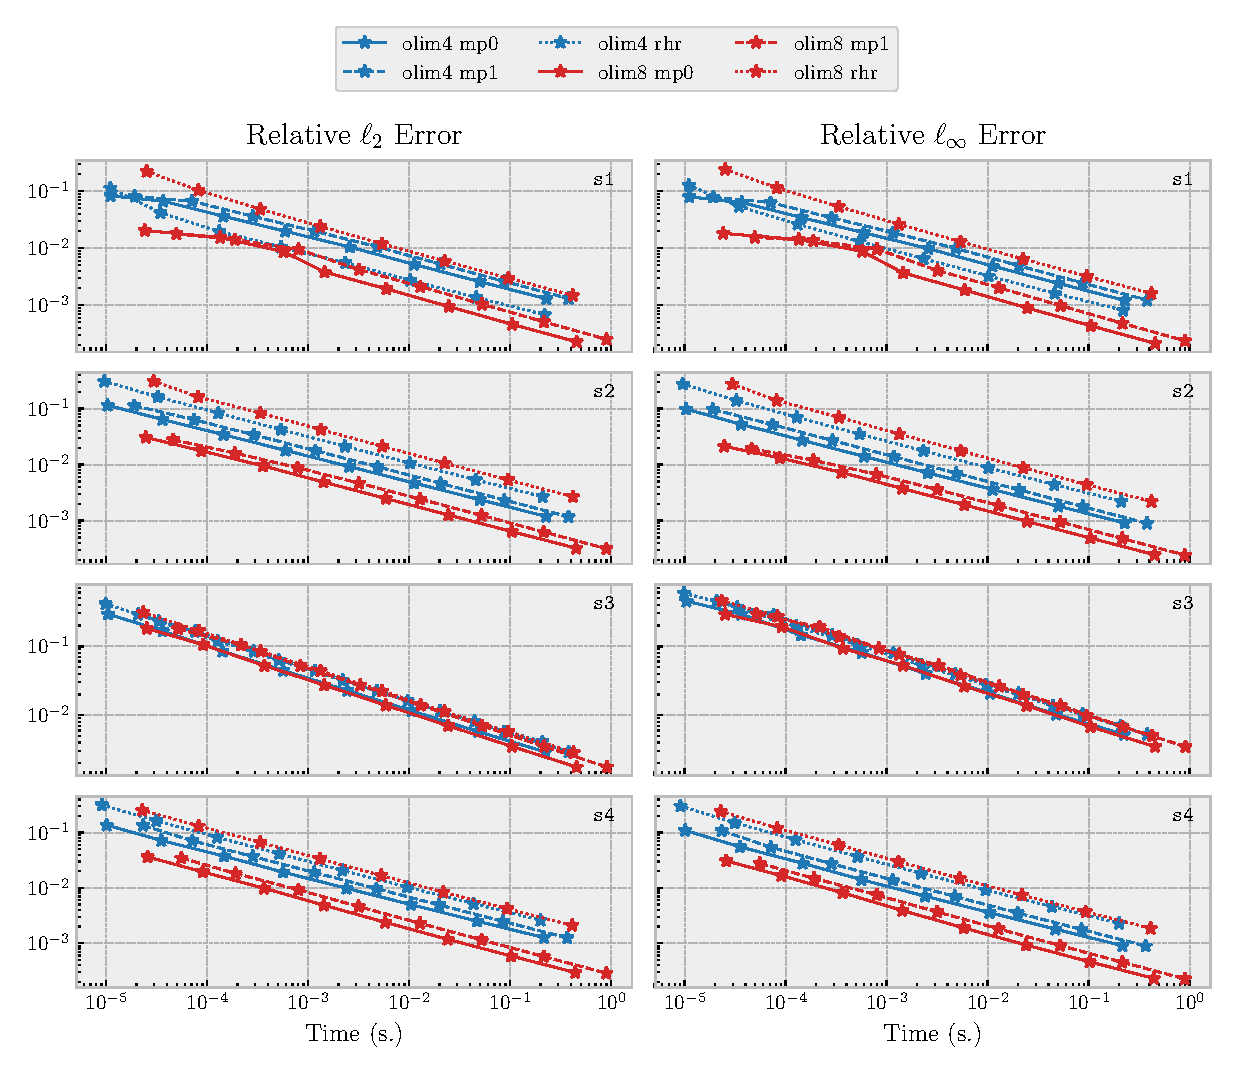
\includegraphics[width=\linewidth]{time_vs_error_2d.eps}
  \caption{\hl{\textbf{TODO}}: $\rfac = 0.1$}
\end{figure}

\begin{figure}[H]
  \centering
  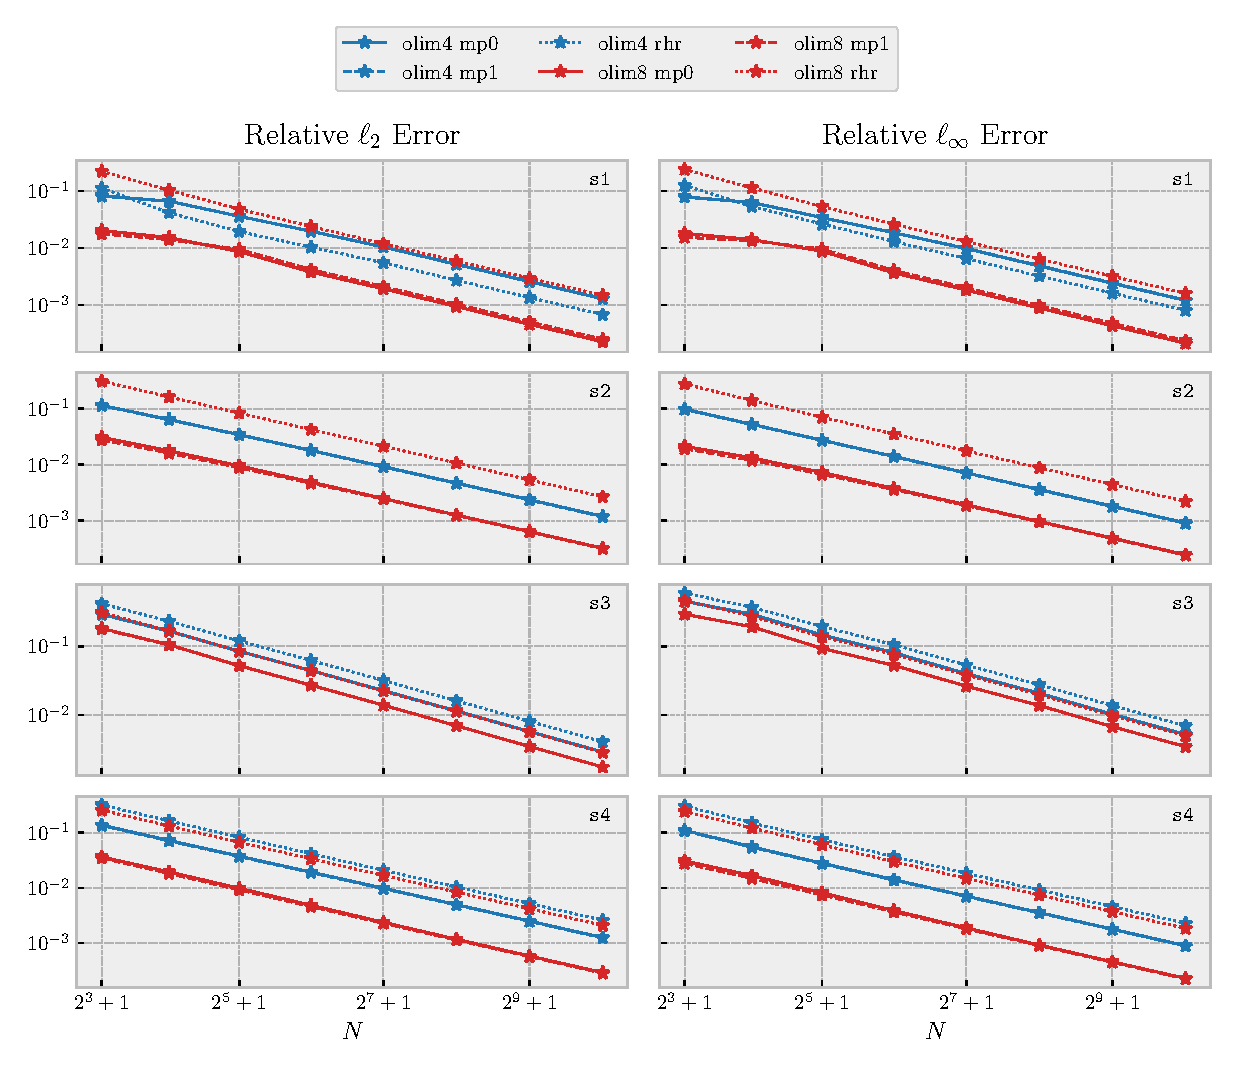
\includegraphics[width=\linewidth]{size_vs_error_2d.eps}
  \caption{\hl{\textbf{TODO}}: $\rfac = 0.1$}
\end{figure}

\begin{figure}[H]
  \centering
  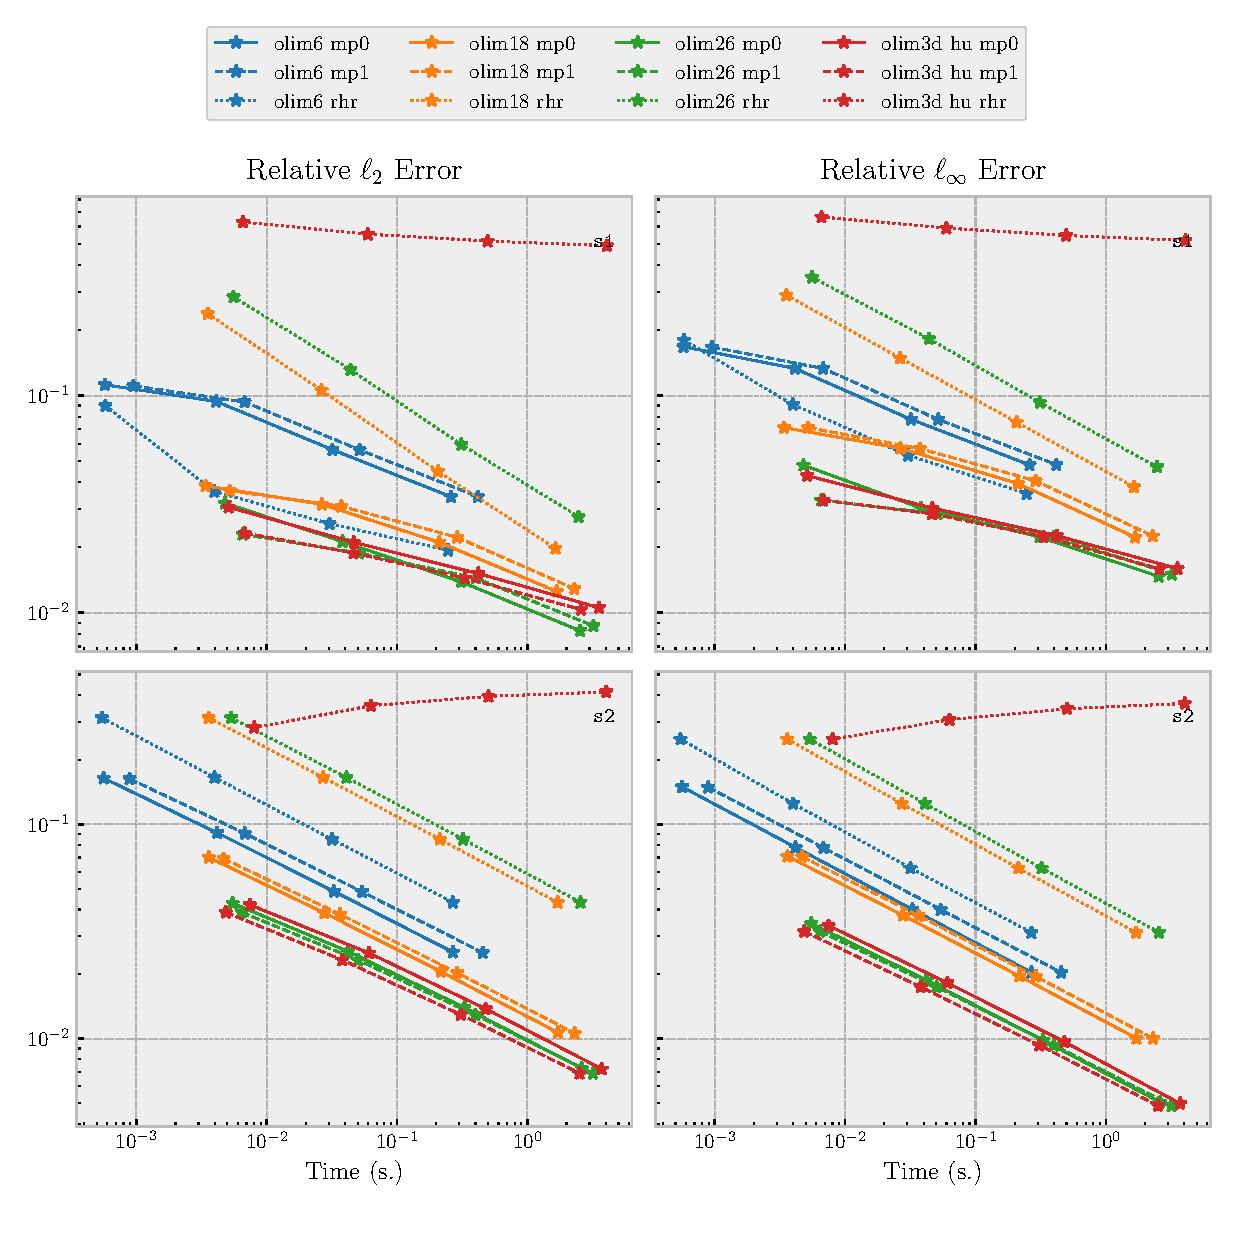
\includegraphics[width=\linewidth]{time_vs_error_3d_part1.eps}
  \caption{\hl{\textbf{TODO}}: $\rfac = 0.1$}
\end{figure}

\begin{figure}[H]
  \centering
  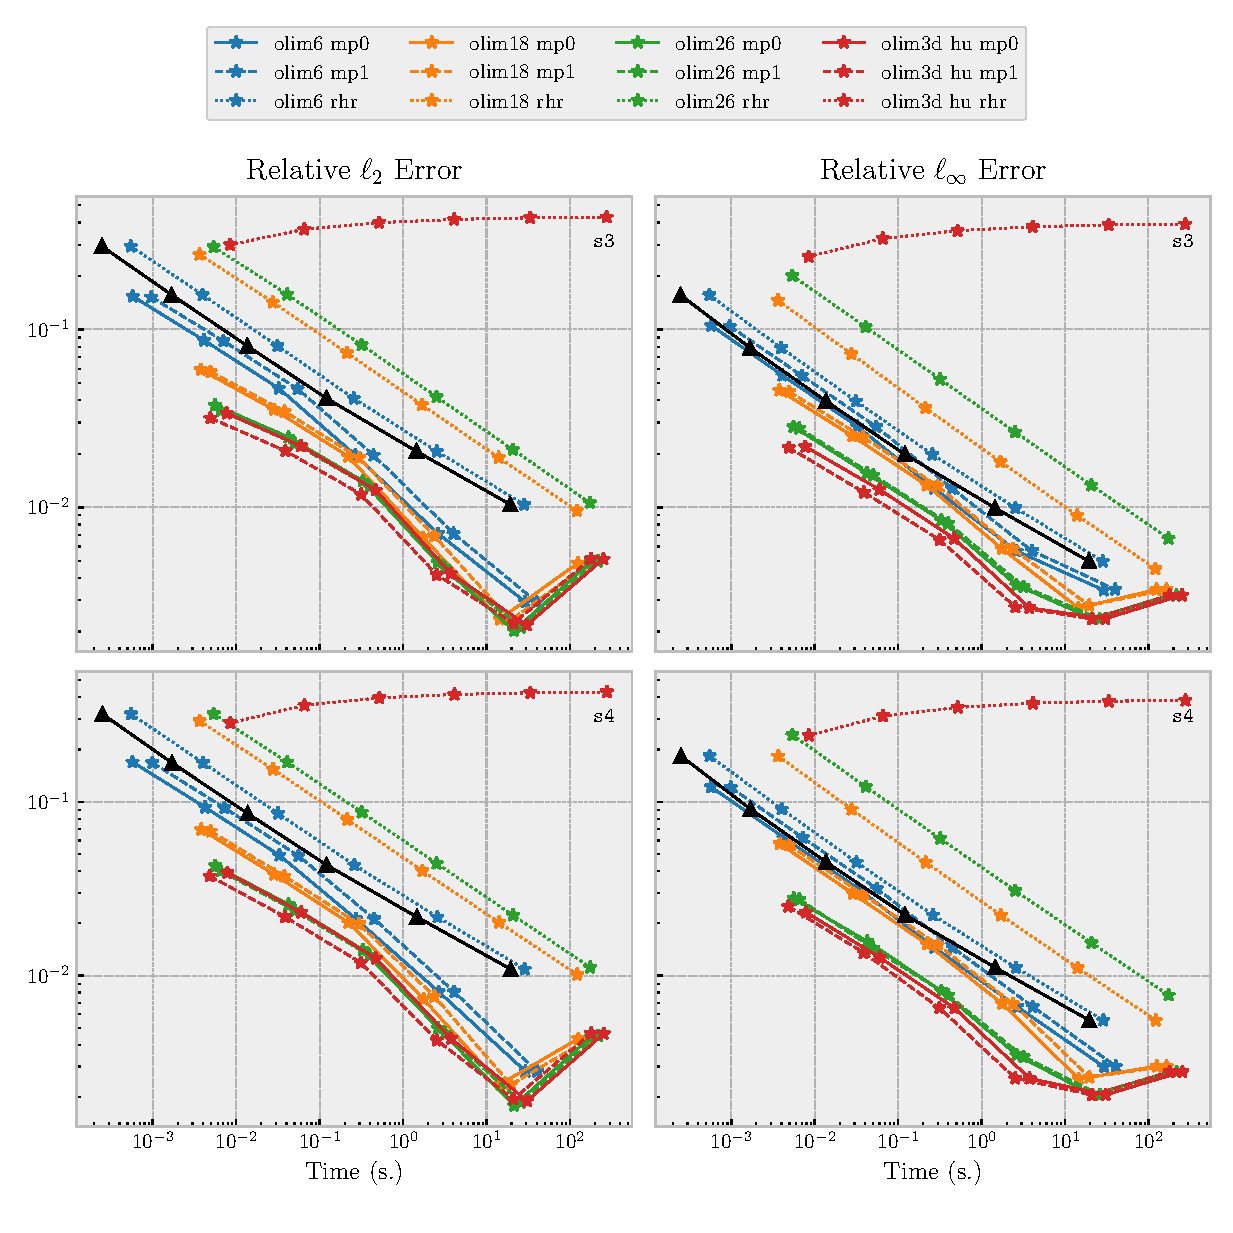
\includegraphics[width=\linewidth]{time_vs_error_3d_part2.eps}
  \caption{\hl{\textbf{TODO}}: $\rfac = 0.1$}
\end{figure}

\begin{figure}[H]
  \centering
  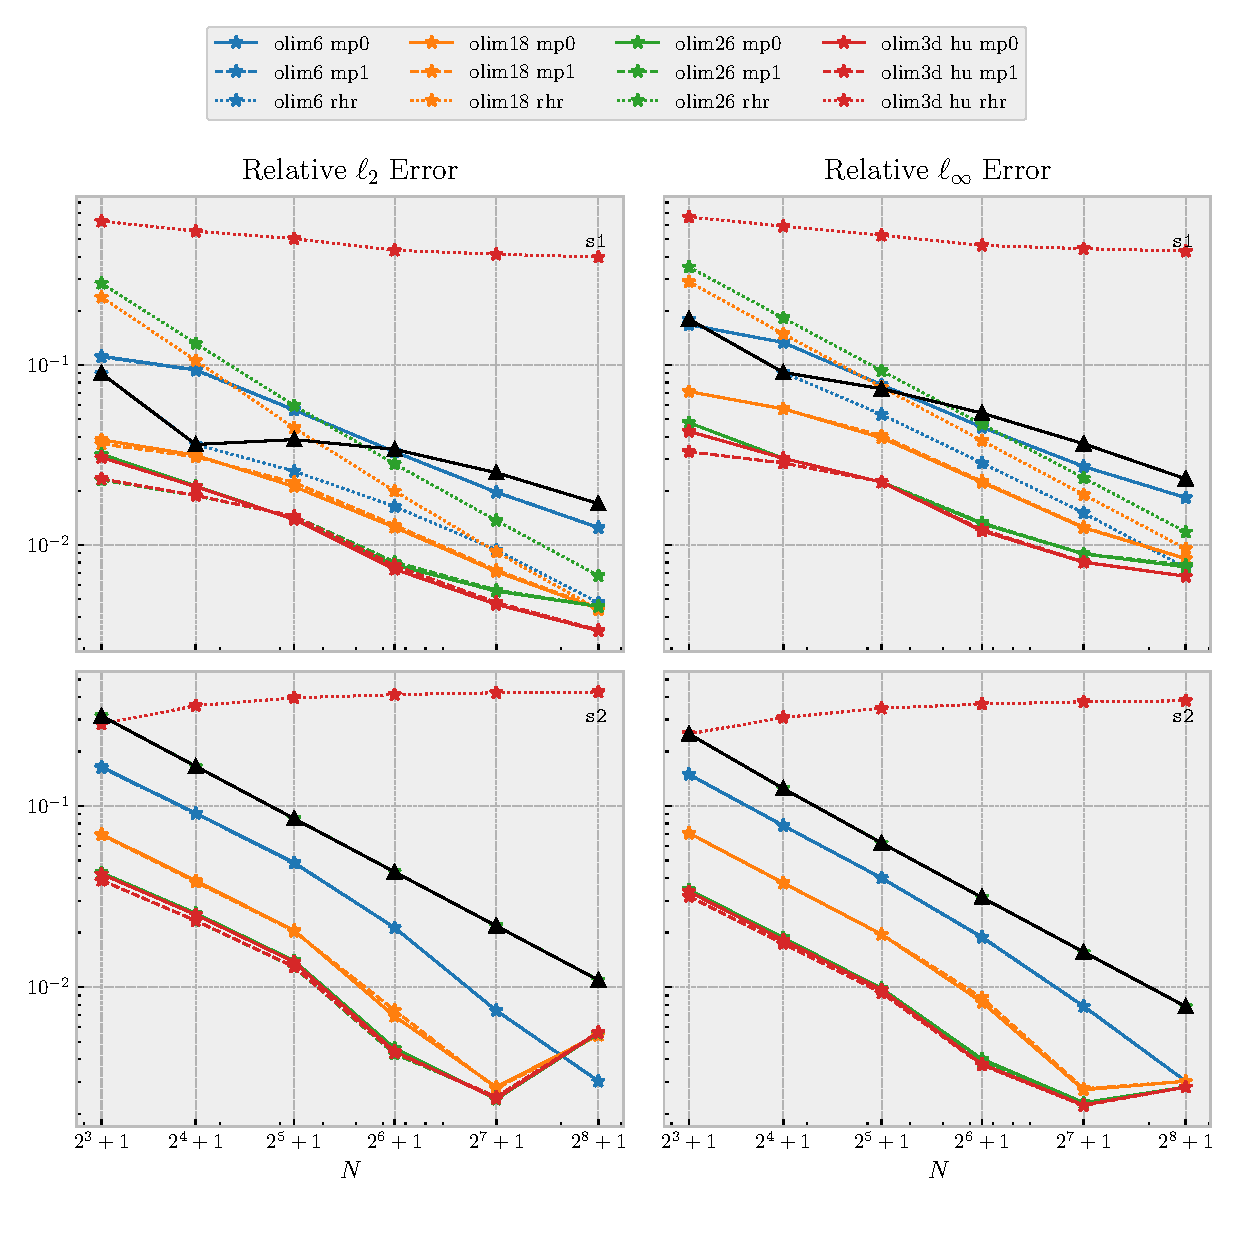
\includegraphics[width=\linewidth]{size_vs_error_3d_part1.eps}
  \caption{\hl{\textbf{TODO}}: $\rfac = 0.1$}
\end{figure}

\begin{figure}[H]
  \centering
  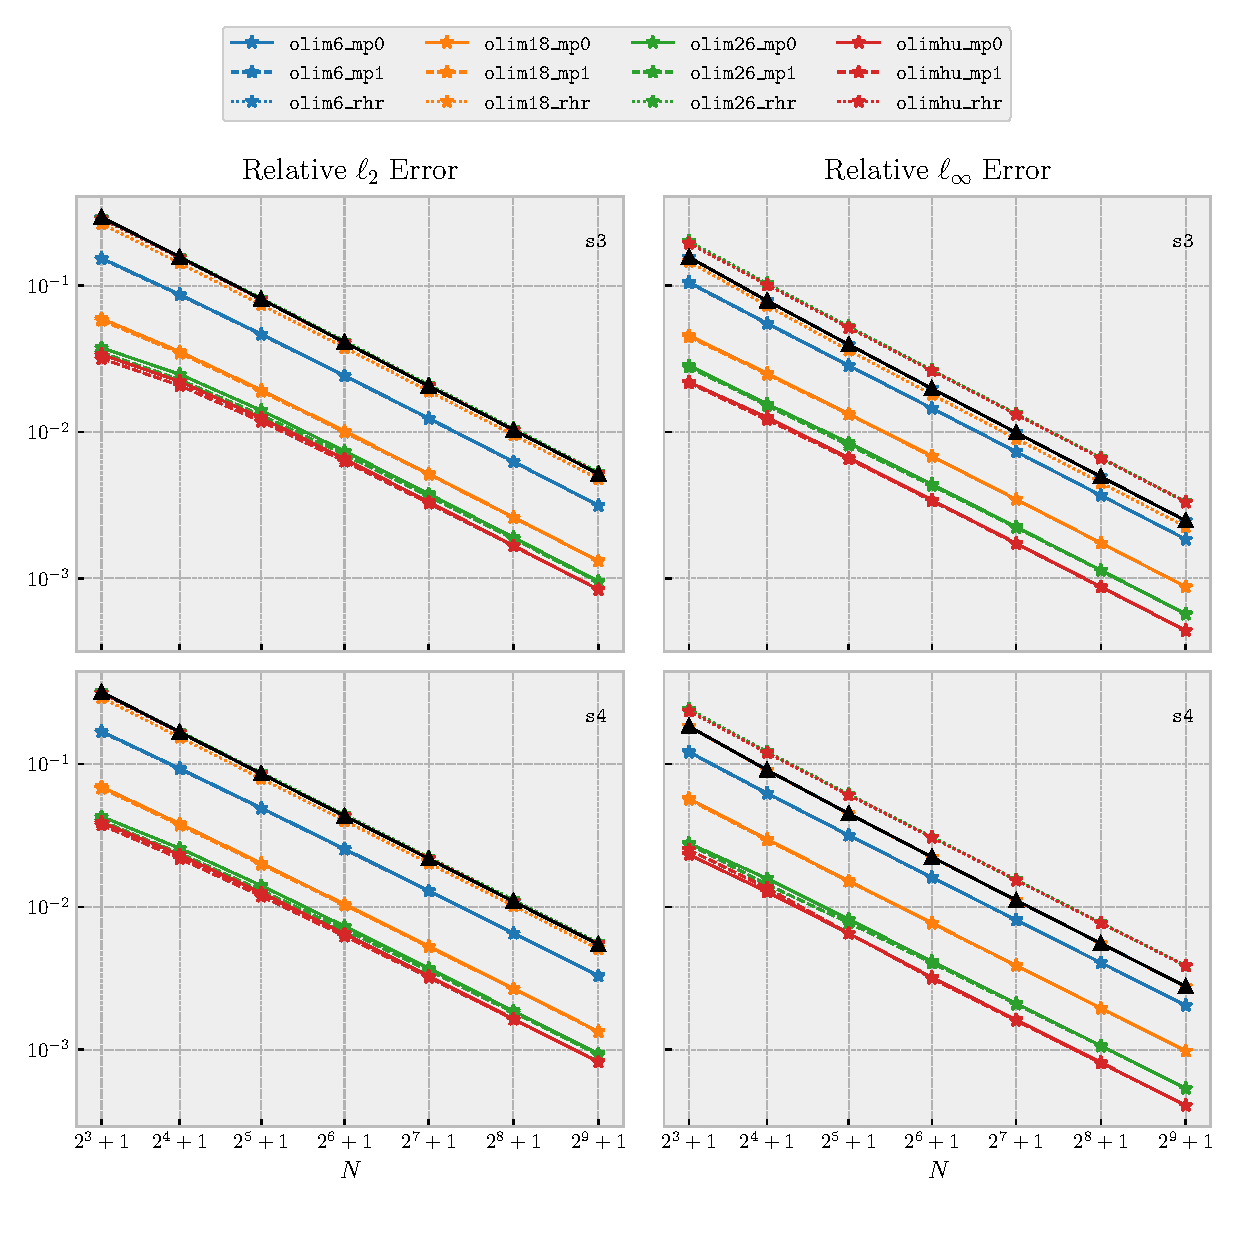
\includegraphics[width=\linewidth]{size_vs_error_3d_part2.eps}
  \caption{\hl{\textbf{TODO}}: $\rfac = 0.1$}
\end{figure}

% \begin{figure}[H]
%   \centering
%   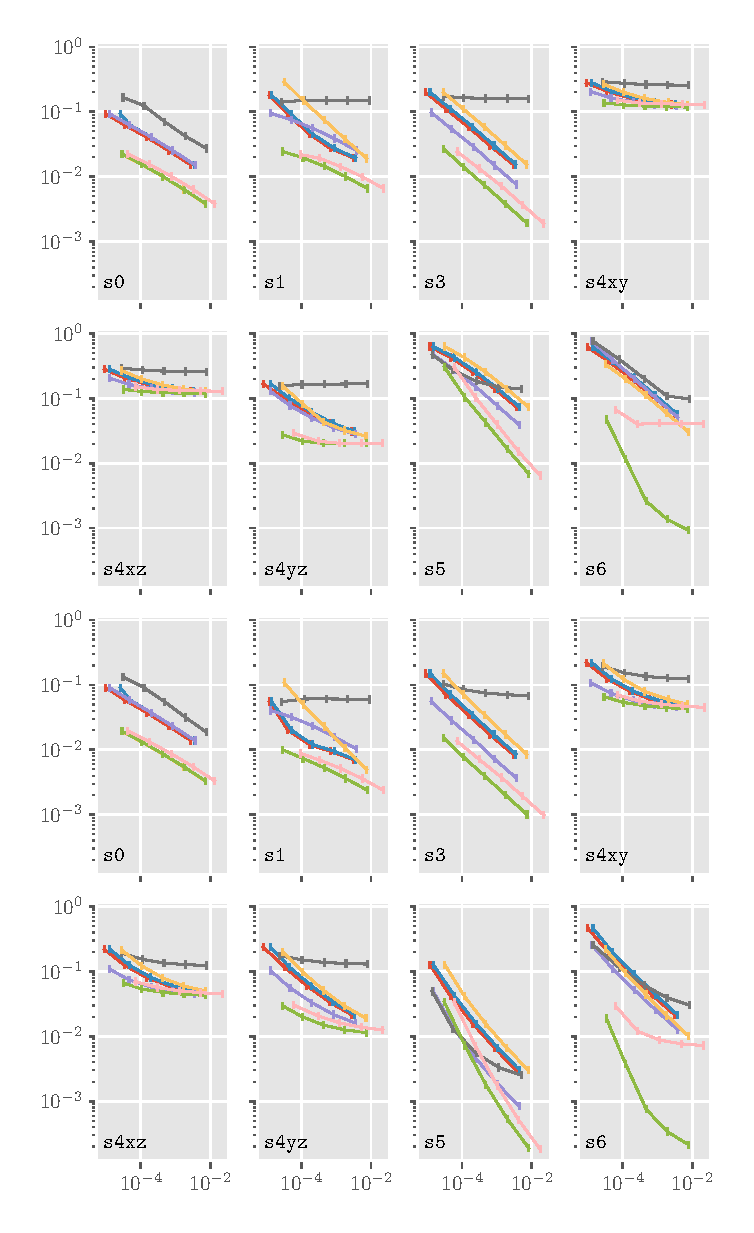
\includegraphics[width=\linewidth]{plots_2d.eps}
%   \caption{\hl{\textbf{TODO}}}
% \end{figure}

% \begin{figure}[H]
%   \centering
%   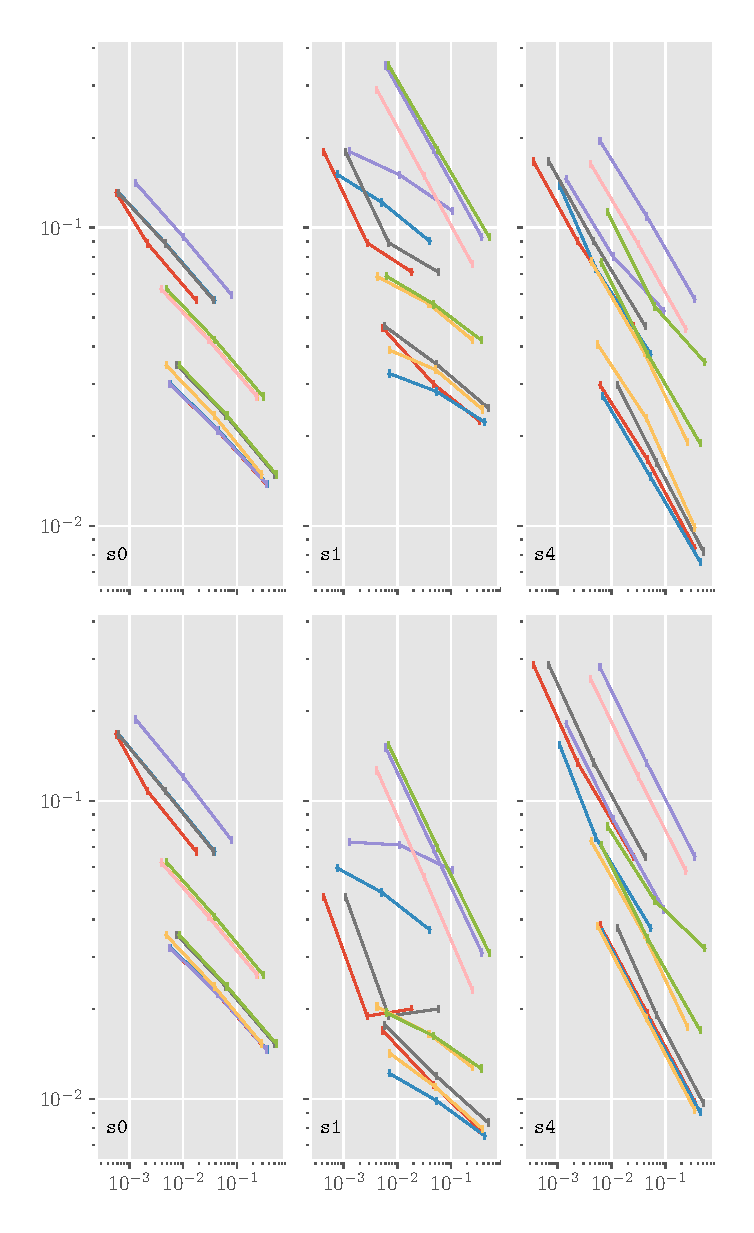
\includegraphics[width=\linewidth]{plots_3d.eps}
%   \caption{\hl{\textbf{TODO}}}
% \end{figure}

% \begin{figure}[H]
%   \centering
%   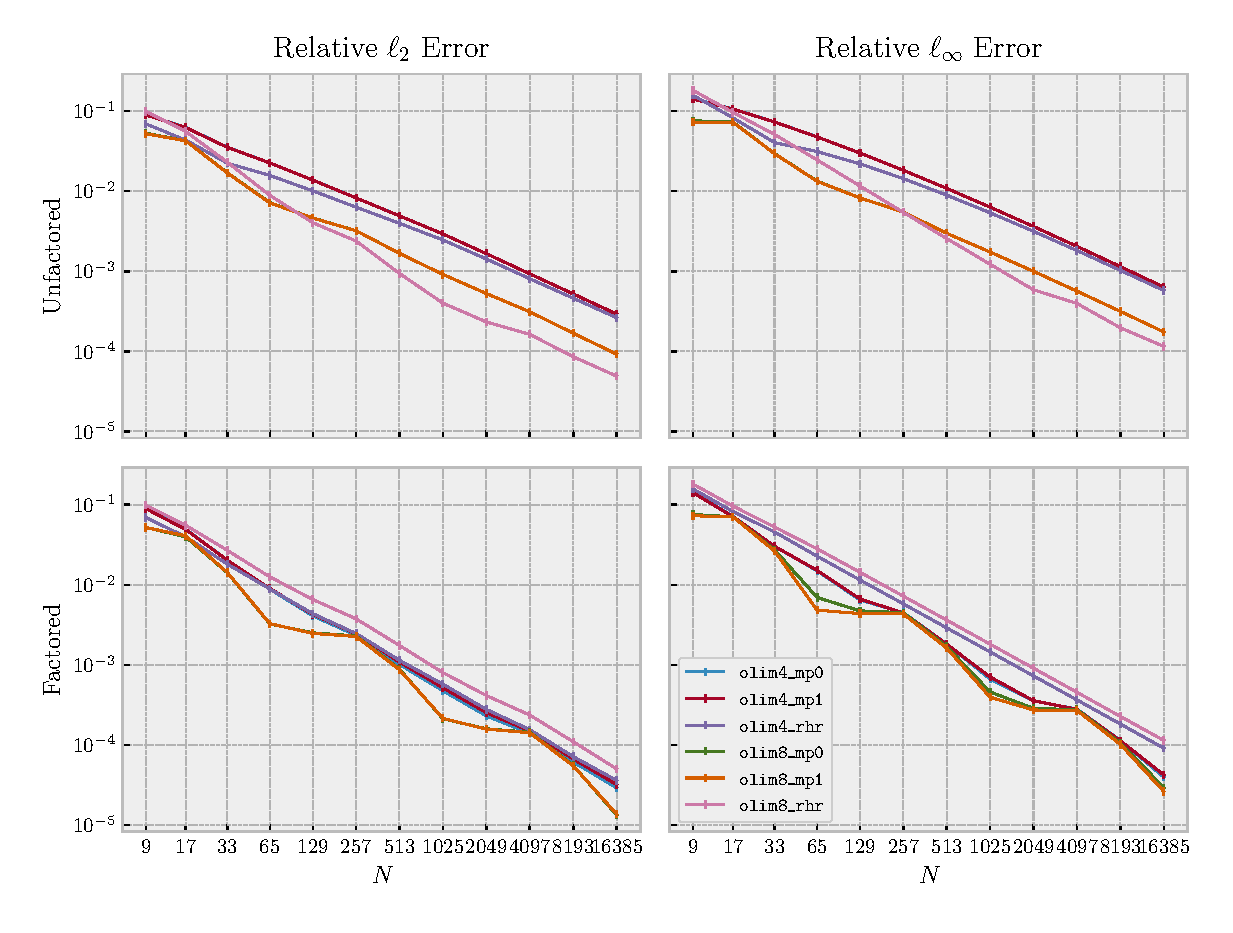
\includegraphics[width=\linewidth]{qv_plots_2d.eps}
%   \caption{\hl{\textbf{TODO}}}
% \end{figure}

% \begin{figure}[H]
%   \centering
%   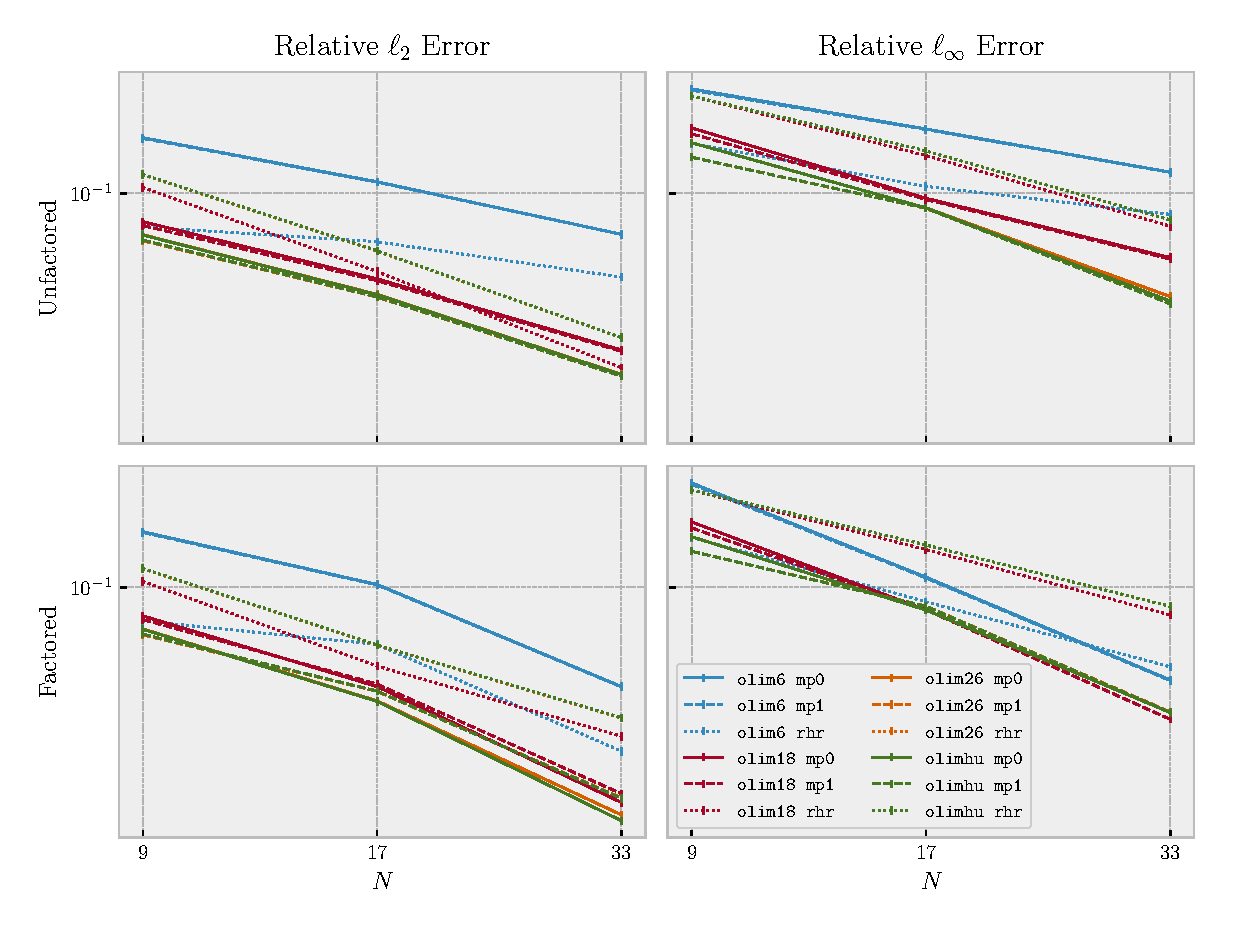
\includegraphics[width=\linewidth]{qv_plots_3d.eps}
%   \caption{\hl{\textbf{TODO}}}
% \end{figure}

% \begin{figure}[H]
%   \centering
%   \includegraphics[width=\linewidth]{factoring_comparison_plots.eps}
%   \caption{\hl{\textbf{TODO}}}
% \end{figure}

\end{document}

%%% Local Variables:
%%% mode: latex
%%% TeX-master: "sisc-eikonal.tex"
%%% End:
